%pose estimation
\chapter{Activity Recognition}
\label{activityRecognition}

\section{Introduction}

In this section we turn to the problem of recognising and clustering various activities across a range of conditions. An activity is a short sequence of motion, typically undertaken by a person, and captured by either video cameras or a motion capture system. Activity recognition is an important field of study, due to the growing demand for systems that can reliably infer behaviour in a range of settings. There are a wide variety of applications for activity recognition systems, for example home based care, gaming, surveillance, and for safety on construction sites, among many more. In home care scenarios, where robots may be employed to care for the elderly or for the disabled, the primary consideration is monitoring the status of the patient to determine whether they are healthy and safe. It may also be necessary for the activity recognition system to determine the current state of the patient so as to control the home. Patients may have dementia or limited mobility and therefore it may be necessary to be able to discriminate between low amplitude and ambiguous motions. We may also wish to employ activity recognition systems at construction sites. On large construction sites there will be a large number of hazards, for example machinery operating, uncovered holes dug in the ground, and materials swinging through the air as it is transported. This clearly presents significant danger to people as they move about construction sites. It is desirable, therefore, to employ systems that are capable of inferring the trajectory and likely behaviour of people and machinery as they move around. Systems that can identify when someone is walking and discern some information from their gait may also be useful in biometric applications, for instance in security systems, or for use with autonomous vehicles to identify the behaviour of pedestrians. \\

A number of reviews have explored the space of activity recognition systems. (Vrigkas et al., 2015) develop a taxonomy human activity recognition schemes. Their research highlights that there are two dominant schemas in the activity recognition literature: unimodal and multi-modal. Unimodal schemas use only one sensory modality, such as an image stream, motion capture data, or an audio stream. Unimodal schemas are exemplified by their focus on \textit{low-level} features, such as space-time events and shape features. Multi-modal schemas, by contrast, are much more \textit{high-level}. They rely on behavioural features, often built from unimodal low-level features. Similarly, multi-modal schemas can employ networks of activity, such as in crowds, to recognise behaviour. We will be focusing almost exclusively on unimodal methods, however for a discussion of multi-modal techniques please refer to (Vrigkas et al., 2015). \\

Perhaps two of the most dominant unimodal activity recognition paradigms are (i) based on the extraction of space-time features and (ii) on the extraction of shape and appearance features. \textit{appearance-based} methods typically extract the silhouette of a moving person before performing further analysis. (bobickdavis2001) formulate a view-specific action recognition method that is invariant to changes in scale and translation of the underlying activity. Their method consists of an initial training phase from which statistical moments are computed from a series of image derivatives. Specifically (bobickdavis2001) compute a motion energy image (MEI) and a motion history image (MHI), which collectively define where and how a motion occurred, respectively. Recognition of a query image given the training data is performed by computing the Mahalanobis distance between the statistical moments of the query MEI/MHI pair and those computed during training. (huangxu2007) attempt to introduce viewpoint invariance by using orthogonal cameras. They align silhouettes extracted from each camera along the medial axis and then extract a set of features. A hidden Markov model is used for training and recognition of the extracted features. This is an extension of the approach by (weinland et al 2006) who use a series of calibrated cameras to extract motion history volumes from the silhouette of an actor as they perform an activity. A Fourier transform is used to learn and compare various activities. While this technique is viewpoint invariant it relies on multiple calibrated cameras, which limits its applicability. A similar approach is taken by (Chakraboty et al 2008) who combine a whole body person detector with a parts based detector that they use as input to a classification algorithm. Furthermore, (Chakraboty et al 2008) use multiple sub-classifiers taken from multiple viewpoints for each body part. A collection of hidden Markov models are trained to identify actions based on the pose of body parts detected in query videos. The use of human silhouettes as the input stage to a recognition algorithm has existed for many years. In 1994 (guo et al 1994) developed a two stage process that first fit a stick-figure model to the silhouette in every frame and then used a neural network to recognise actions based on the changes to the stick-figure parameters over time. Similarly, (niyogianderson1994) extract edges from the spatio-temporal volume of a walking person, from which they extracted bounding contours. A nearest neighbour approach was used to measure the distance between spatio-temporal contours from various subjects in order to assess similarity. This algorithm is not view invariant as they required that the subjects moved parallel to the image plane. A multi-view appearance based technique was introduced by (qhu et al 2013) which uses random forests (breiman2001) to map silhouettes to activity classes.\\

In contrast to the methods introduced above, \textit{space-time} methods predominantly rely on optical flow information rather than appearance cues. As with all activity recognition techniques they must deal with two problems: (\textit{i}) view invariance and (\textit{ii}) rate invariance. View invariance describes the ability of an algorithm to recognise activities from any arbitrary viewpoint. This is obviously an extremely important characteristic, as it is only in very controlled situations that an activity would be performed from a consistent viewpoint. Biometric scanners may, for instance, require a gesture to be performed to allow access, however even in this situation there would be a distribution of viewing angles from which an action could be observed. In contrast, a surveillance system may need to be able to determine the gait of a person as they walk in any direction relative to the camera viewpoint. Similarly, in augmented reality gaming there is no fixed orientation for which actions are performed (i.e the participant does not have a screen to face) and therefore gestures could be performed in any arbitrary orientation relative to the cameras. Rate invariance, which refers to the speed at which an activity is performed, is another important consideration. Walking, for instance, is not necessarily simply slow running. Two subjects may therefore walk at different speeds and we would expect that suitably discriminative algorithms would be able to identify the difference between them. This is a non-trivial problem, however, and is in general NP-hard (check this). Fortunately there exist a number of algorithms for rate invariant activity recognition that are computationally feasible. The algorithms we examine deal with these two problems to varying degrees. (Vrigkas et al 2013) extract motion trajectory curves from optical flow data. As is common with almost all the frameworks mentioned in this thesis they require that a model is learnt to discriminate between various activity classes. During learning they use Gaussian mixture models to cluster motion curves into distinct classes. They then compare and contrast various schemes for matching the clustered motion curves, including: \textit{longest common subsequence} and \textit{canonical time warping}. Time warping algorithms, commonly known as dynamic time warping (DTW) are popular for matching time series data, as they permit sub-frame comparisons between sequences. (Zhous and de la torre 2009) developed a \textit{canonical} version, which allows for matching between two signals of different dimensionality. In an extension of this work (Zhous and de la torre 2012) develop a generalised time-warping algorithm which allows for matching between signals of different modalities using a feature weighting layer and has a linear complexity, as opposed to quadratic complexity, which is the norm for most algorithms. (Make note of the fact that this work allows for comparisons between different modalities?). A probabilistic version of dynamic time warping was introduced by (Yamata et al 2012). They use the squared loss mutual information to measure the statistical dependency between two sequences. A systematic analysis of the influence of changing the execution rate of an activity was performed by (Veeraraghavan et al 2009). They learn a generative model of activities which includes a probabilistic model of the function space characterising the various temporal warpings of any activity. This allows for a computationally efficient inference algorithm for action recognition and gait-based person identification with time-warped activity profiles. While most techniques first extract features from signals and then use dynamic time warping to match various signals to each other, (Seto et al 2015) instead use dynamic time warping to define templates from signals, which are then used as input to a matching algorithm. \\

So far we have only discussed the case where the actions of a single subject are recognised. (Parkagarwal2003) use a hierarchical Bayesian network to model the interactions between two interacting subjects. They extract features from a sub-person level, a single person level, and from the interaction of the two subjects. (Yun et al 2012) evaluate the discriminative ability of various features, such as depth and stereo information, for recognising interactions between multiple people. Notably, they find that features based on the distances between joints offer the strongest recognition performance. 


Their method is powerful as it can handle sequences performed at varying speeds, as opposed to many methods which presume relatively consistent actions.























\section{Motion Capture Data}

We are interested in matching time-series signals of various human activities. We are using motion capture data from the Carnegie Mellon dataset, which includes a wide range of activities, for example: walking, running, dancing, climbing over obstacles, swimming motions, getting up off the ground and sweeping motions. The motion capture data contains the angle of each joint over time, as well as the spatial coordinates of a root node. In order to situate our synthetic examples, we first show some examples of real motion capture data. The first two examples, shown in Fig. \ref{getting_up} are of a subject getting up off the ground from a lying position. The second two examples, shown in Fig. \ref{walks} are of a subject walking in a normal fashion. The goal of our algorithm is to measure the similarity between any two motion inputs. We show that our HSIC measure is capable of discriminating between various motions, however we typically require that the motion is first projected into a lower dimensional space. Before we demonstrate our results we will first give an overview of principle component analysis.\\

In many cases our data will lie in a high-dimensional space. Our input motion capture data, for example, has 59 components, six of which describe the position of the root node over time, while the rest describe the angles of various body joints. There is one joint angle per degree of freedom for each particular joint, however not all joints have the full three degrees of freedom. The joint names and the numbers of degrees of freedom are specified in Fig. {mocap image}.\\

\begin{figure}[h]
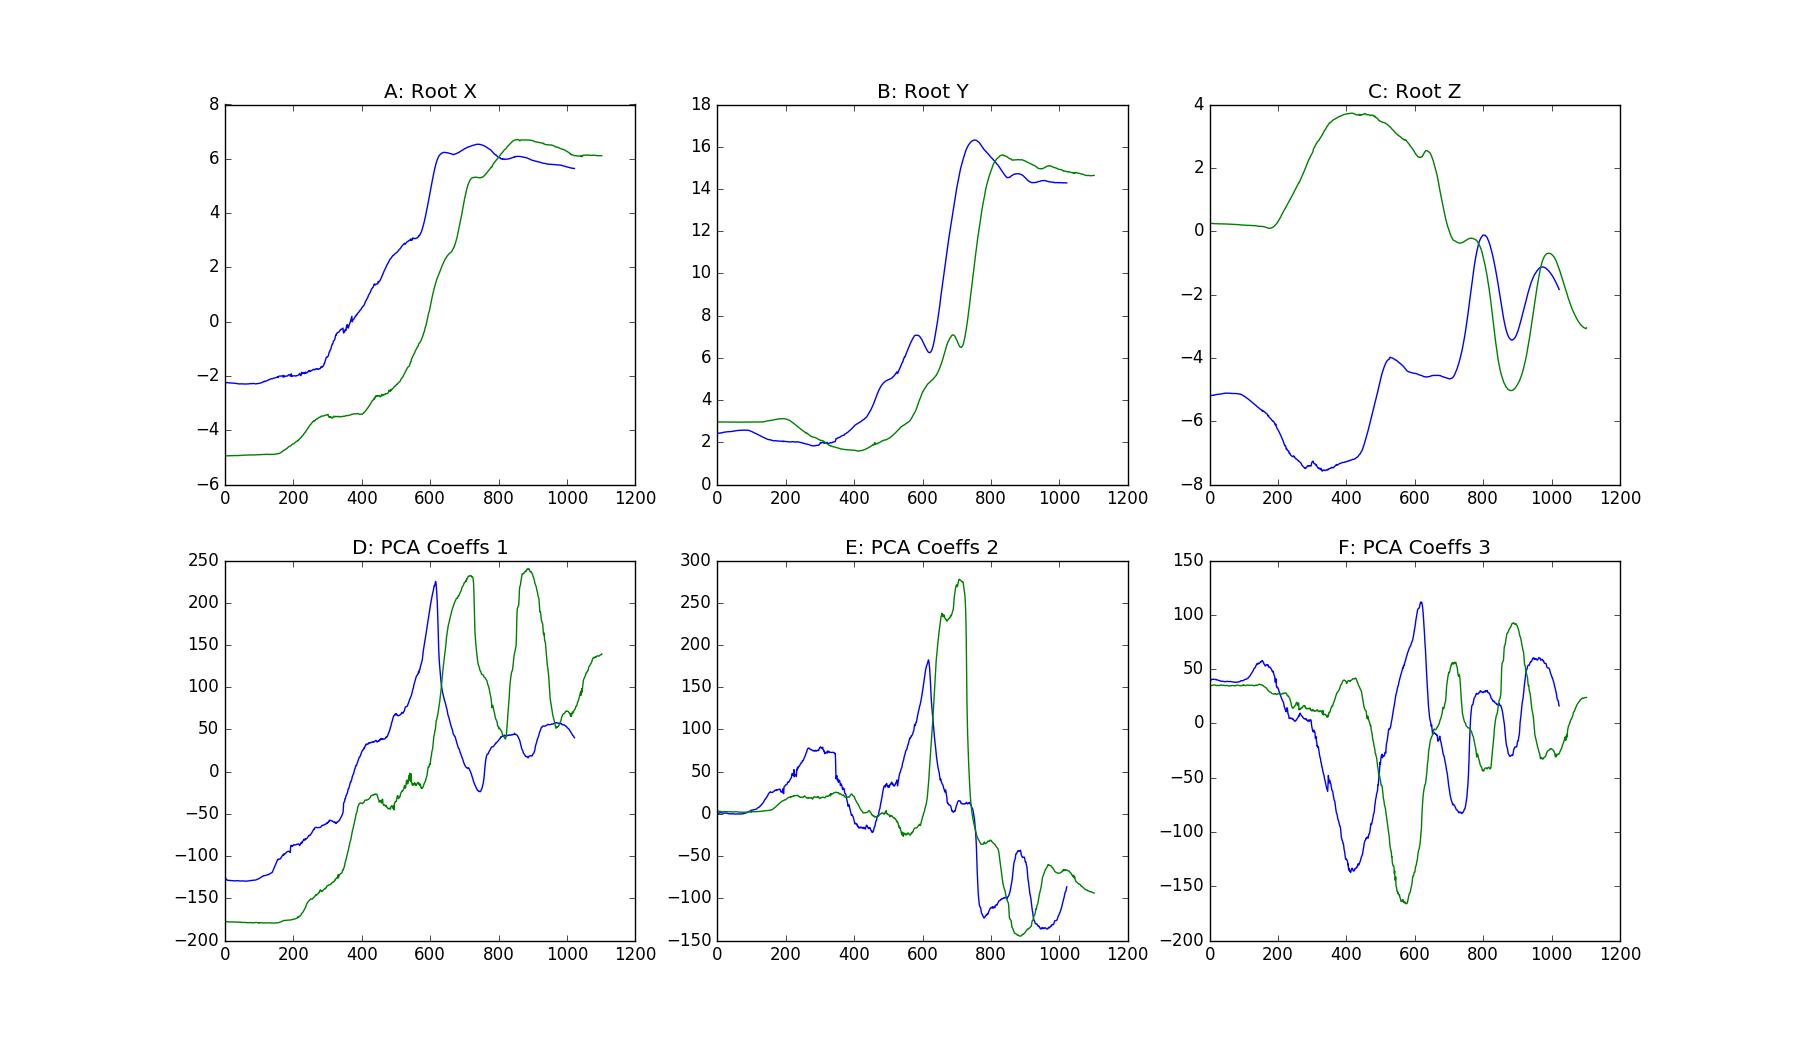
\includegraphics[width=\textwidth]{/home/cshome/j/jcampbell/Desktop/Thesis/Thesis/images/getting_up.png}
\caption{Motion capture data for a subject as they rise from the ground in two 	different examples. The top row shows the position of the root node of the subject while the bottom row shows the data projected according to the PCA basis functions, for each of the first three most significant components. In each of the plots the blue trace is for the first example while the green trace is for the second example. The same subject performed both actions. The two motion examples are 3 and 4 for subject 140 of the CMU Mocap database. \label{getting_up}}
\end{figure}

\begin{figure}[h]
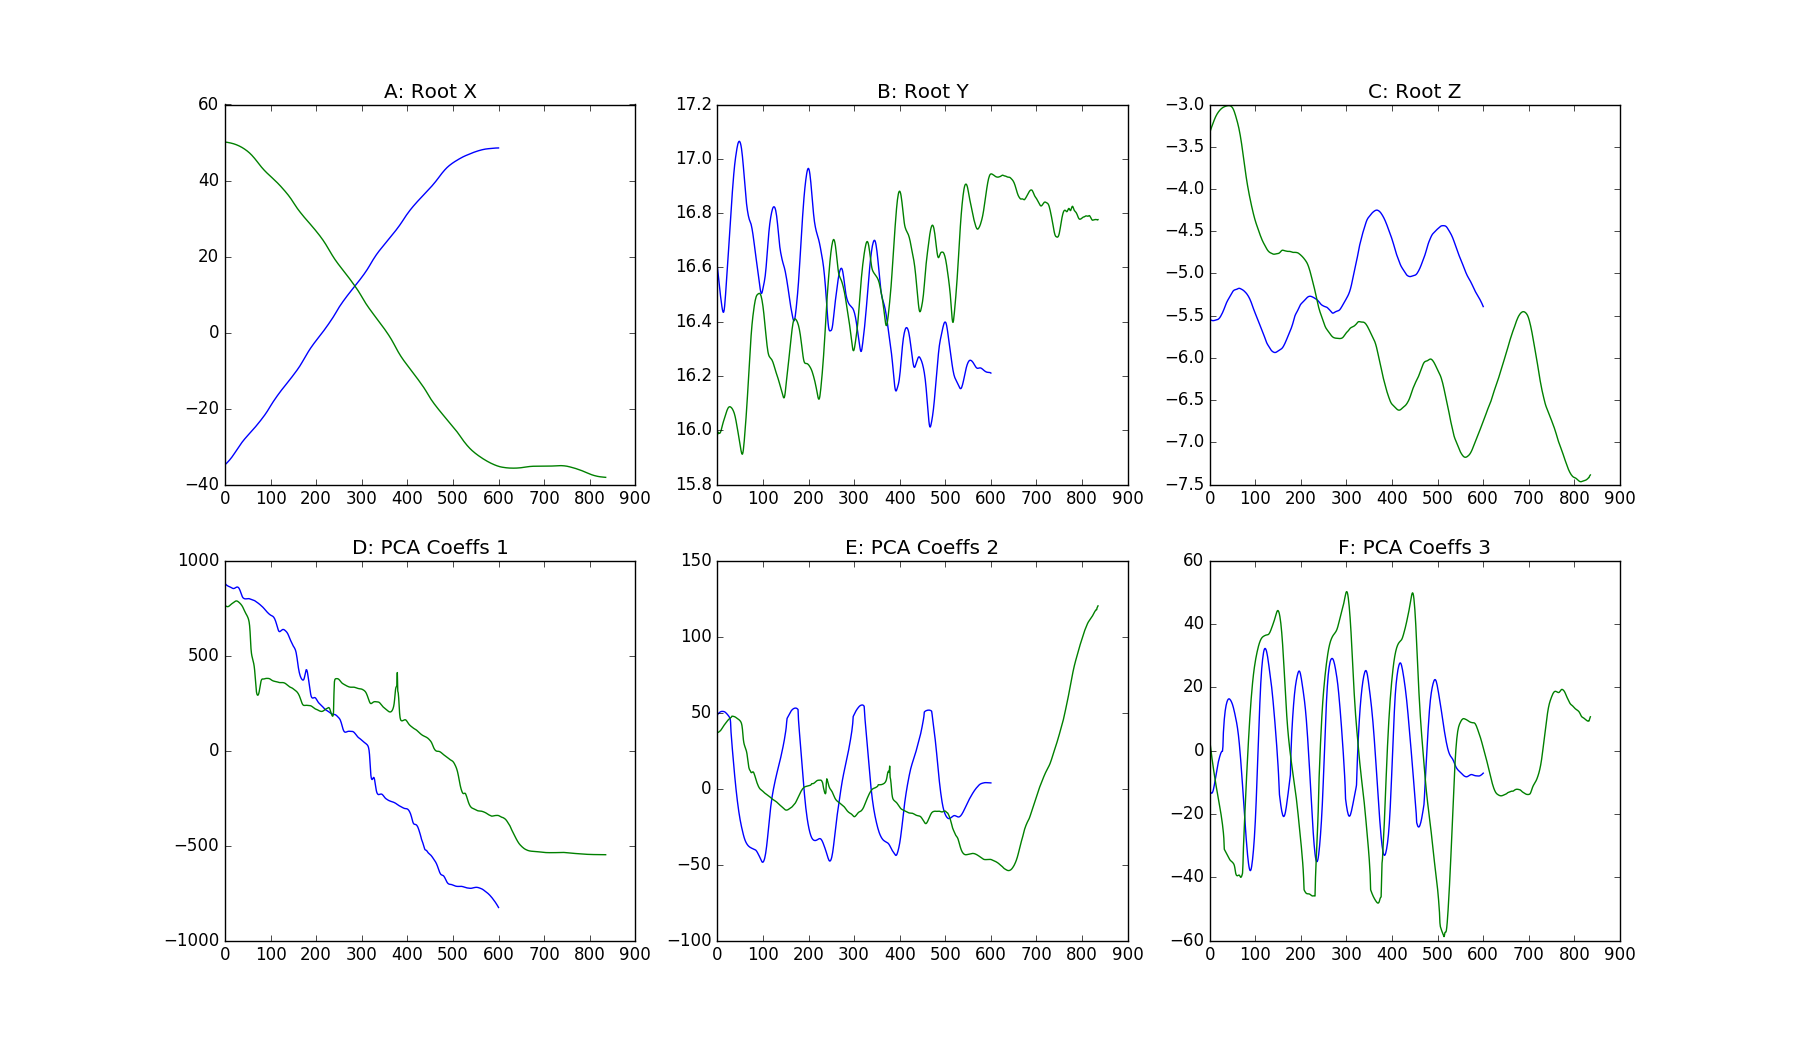
\includegraphics[width=\textwidth]{/home/cshome/j/jcampbell/Desktop/Thesis/Thesis/images/walks.png}
\caption{Motion capture data for a subject as they walk in two different examples. In both cases the subject walked for a short period in one direction and then turned and walked back. The top row shows the position of the root node of the subject while the bottom row shows the data projected according to the PCA basis functions, for each of the first three most significant components. In each of the plots the blue trace is for the first example while the green trace is for the second example. The same subject performed both actions. The two motion examples are 21 and 22 for subject 136 of the CMU Mocap database. \label{walks}}
\end{figure}

\subsection{Principle Component Analysis}

Principle component analysis (PCA) is a widely used method for computing a low dimensional representation of data. Given an $n\:\:\text{x}\:\:m$ data matrix $X$, PCA finds a linear transformation to a new set of coordinate axes such that the variance along each of the new axes is maximised. Typically singular value decomposition (SVD) is used to find this transformation. The PCA transform using SVD performs a factorisation of the data matrix according to

\begin{equation}
X = U \Sigma V^{T} 
\end{equation}

\noindent where $U$ and $V$ are the left and right singular vector matrices of size $n\:\:\text{x}\:\:n$ and $m\:\:\text{x}\:\:m$ respectively. The matrix $\Sigma$ is an $n\:\:\text{x}\:\:n$ diagonal matrix containing the $n$ singular values of $X$. The vectors of $V$ are eigenvectors of the covariance matrix $X X^{T}$ and represent the principle components of the transformed data. We transformed data matrix is found by projecting the original data matrix into the space defined by the PCA axes according to

\begin{equation}
Y = V X. 
\label{PCA_compute}
\end{equation}

This method, however, only works efficiently in cases where the dimensionality of each sample is much lower than the number of samples available, i.e. when $n > p$. This is because the covariance matrix $X X^{T}$ becomes very large. \\

It is often the case where the dimensionality of our samples is much greater than the number of samples available. We will see in later sections that this is the case for temporal synchronisation of videos. If we represent each frame of a video as a single vector then the dimensionality of each sample is equal to the number of pixels in the image. If our video is only 100 - 200 frames long, then we clearly have $p >> n$. In this situation we turn to an alternative method for estimating the principle components, as defined by reference. \\

Since the number of samples is low we can efficiently compute the alternative covariance matrix $X^{T} X$ which is of size $n\:\:\text{x}\:\:n$. We then compute the eigenvalues and eigenvectors of this covariance matrix. The matrix $V$ is formed by stacking the eigenvectors in columns according to the size of the corresponding eigenvalues and can then be used as in Eq. \ref{PCA_compute}.\\

\section{Synthetic Function Matching with HSIC}

The principle contribution of this section is to demonstrate that our HSIC based measure provides a robust measure of the similarity between two arbitrary time-series signals. We demonstrate this capability with a series of examples on synthetic data. As a further proof of concept we also demonstrate that our measure could be used to re-construct a signal from data, in cases where Fourier based methods are not suitable. \\

We saw in Figs \ref{getting_up} and \ref{walks} that our input is a multi-dimensional time-series signal. The top rows of each of these figures are raw input data, while the bottom rows are the PCA transformed data. In each plot we have traced a single parameter from each of two motions. Our input is given by the variables $X = \{x_0, x_1, ..., x_n\}$ and $Y = \{y_0, y_1, ..., y_n\}$, where each of the $n$ samples $x_i$ and $y_i$ are vectors of length $m$. Each element $x_{ik}$ and $y_{ik}$ of $x_i$ and $y_i$ gives the value of a single parameter at a single point in time. It may be, for example, that $x_i$ and $y_i$ are pixel intensities, spatial coordinates of a point on a moving target, or joint angles from motion capture data. As usual we have that $\text{HSIC}(X, Y) = \frac{1}{n^2}\text{tr}\textbf{(KHLH)}$ where $\textbf{H}$ is a centering matrix and $\textbf{K}$ and $\textbf{L}$ are Gram matrices defined on $X$ an $Y$ respectively. As before, our kernel matrix is defined as

\begin{equation}
\textbf{K}_{i,j} = k(x_i,y_j) = \exp^{-((x_i-y_j)\Sigma(x_i-y_j)^T)}
\end{equation}

\noindent where $\Sigma$ is a covariance matrix.\\

Before we begin a discussion of further experiments we first introduce our normalised version of the HSIC, which we term NHSIC. The NHSIC is defined as 

\begin{equation}
\text{NHSIC}(X,Y) = \frac{\text{HSIC}(X,Y)}{\sqrt{\text{HSIC}(X,X)\text{HSIC}(Y,Y)}}
\end{equation}

\noindent and is necessary because, as we will see, we need to vary the choice of (co)-variance for any choice of $X$ and $Y$. We therefore need to scale the HSIC value in order to be able to compare any two results. This will be elaborated further below. \\

In previous works a number of authors have used the median of the data values as the variance in the kernel function. We show instead that it is better to estimate the (co)-variance from the data. This produces much more stable results than the median value, which is important if we are using the NHSIC as an energy measure in an optimisation schema. In Fig. \ref{var_med} we show how the choice of variance affects the HSIC between a fixed signal and a signal with a varying amplitude. In the left plot we can see that the NHSIC varies smoothly with changes in the amplitude of the test signal, while in the right plot the NHSIC results are noisy and contain a significant number of local minima.\\

\begin{figure}[h]
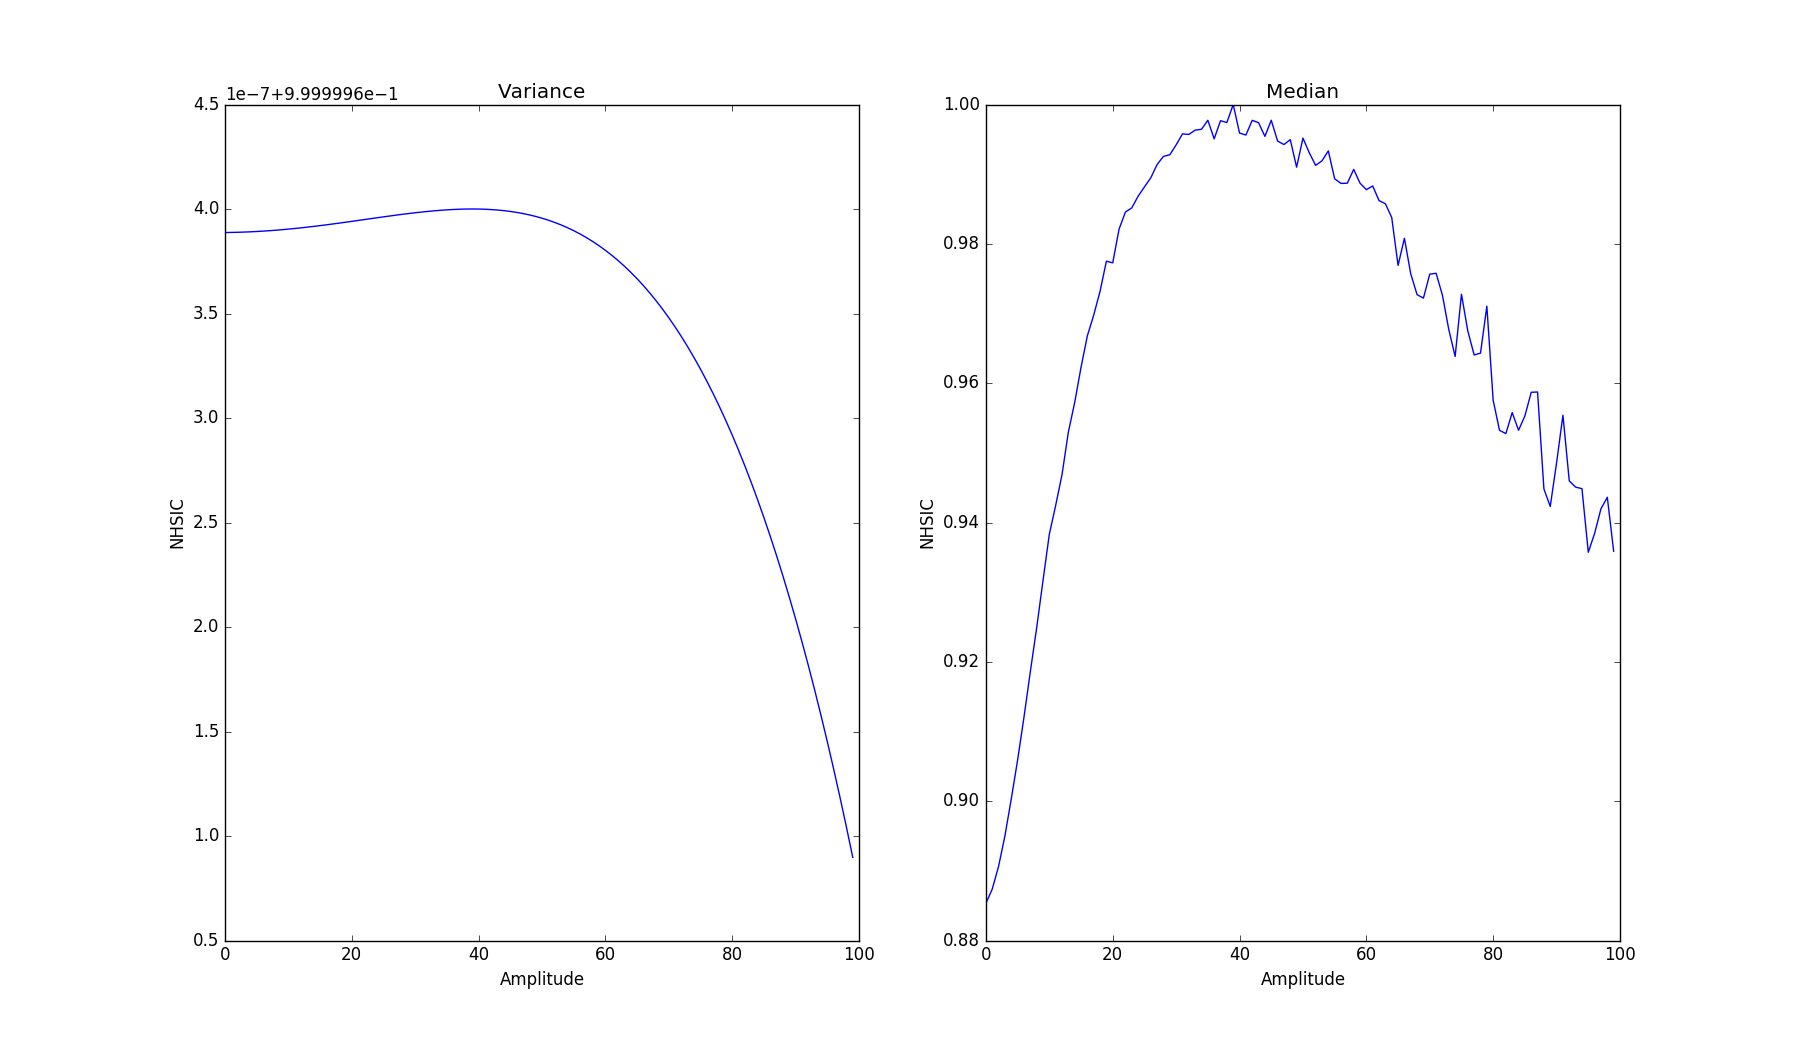
\includegraphics[width=\textwidth]{/home/cshome/j/jcampbell/Desktop/Thesis/Thesis/images/var_med.png}
\caption{NHSIC results using the variance estimated from data (left plot) and the median of the values (right plot) to measure the similarity between a signal with a fixed amplitude and another with a varying amplitude. It is difficult to see in the left plot however the maximum value 9at index 39) is correct, as is that for the right plot.  \label{var_med}}
\end{figure}

One of the consequences of performing computations on sine waves is that the variance of the signal increases quadratically with linear increases in the amplitude. This effect can be seen in Fig. \ref{amp_var} which demonstrates the changes in variance as the amplitude of a sine wave increases. If we were to choose a fixed value for the (co)-variance in the kernel function, then we would effectively be restricting the domain of the kernel function given the variance of the input signal. At first glance this would seem fine, as it is our goal to discover differences in two signals, which will clearly be uncovered if our kernel function treats signals with different variances differently. The problem, however, is that as the magnitude of a sine wave approaches infinity, the HSIC will approach a value of one. This means that a signal with a large amplitude is deemed more similar to a reference signal than the reference signal with itself. If we are given the three functions: $f_1(x) = 0.9\sin(x)$, $f_2(x) = 0.25\sin(x)$, and $f_3(x) = 2.5\sin(x)$, with the goal of asking which of $f_1$, $f_1$, or $f_1$ is most similar to $f_{\text{ref}}(x) = \sin(x)$, then we would be given $f_3$ as the closest match. Notably, if the (co)-variance of the kernel function is fixed, then we would have that $\text{HSIC}(f_{\text{ref}}, f_3) > \text{HSIC}(f_{\text{ref}}, f_{\text{ref}})$. Thankfully the solution to this problem is very simple: we require only that the variance of the kernel function be estimated independently for any HSIC computation. As mentioned previously, however, this means that we must also normalise the resulting HSIC value.  \\

In Figs. \ref{fixed_var_no_norm}, \ref{floating_var_no_norm}, \ref{fixed_var_normalisation}, and \ref{floating_var_normalisation} we show the effect of computing the HSIC between two sine waves, one with varying amplitude and frequency, under a number of different conditions. In all four of these experiments the same test sine wave was used. In Figs. \ref{fixed_var_no_norm} and \ref{floating_var_no_norm} the incorrect result is returned, while in Fig. \ref{fixed_var_normalisation} the correct result is returned, however it is less distinct than the (correct) results in Fig. \ref{floating_var_normalisation}. It is difficult to see in these examples, however the correct frequency is obtained for almost all magnitudes. In Fig. \ref{freq} we can see that at the correct magnitude the correct frequency is clearly found by our algorithm. 



\begin{figure}[h]
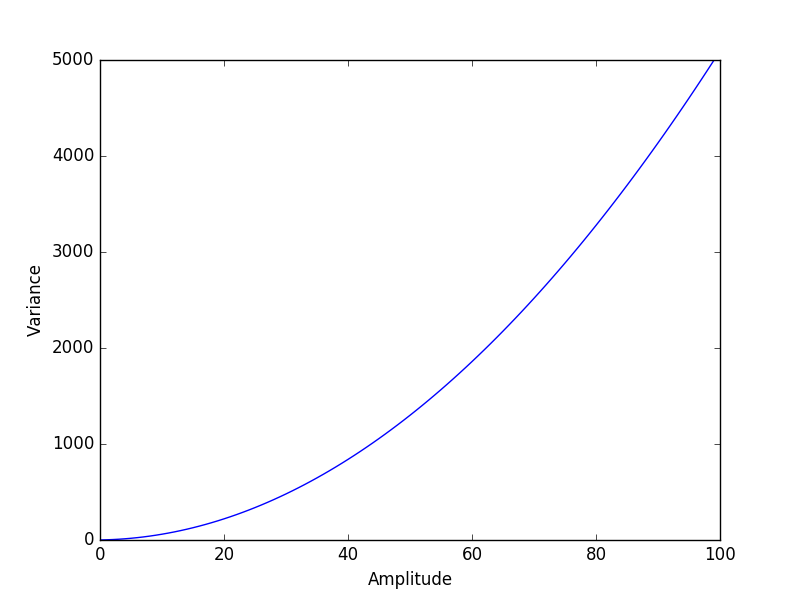
\includegraphics[width=\textwidth]{/home/cshome/j/jcampbell/Desktop/Thesis/Thesis/images/amp_var.png}
\caption{Variance of a sine wave as the amplitude is linearly increased.\label{amp_var}}
\end{figure}

\begin{figure}[h]
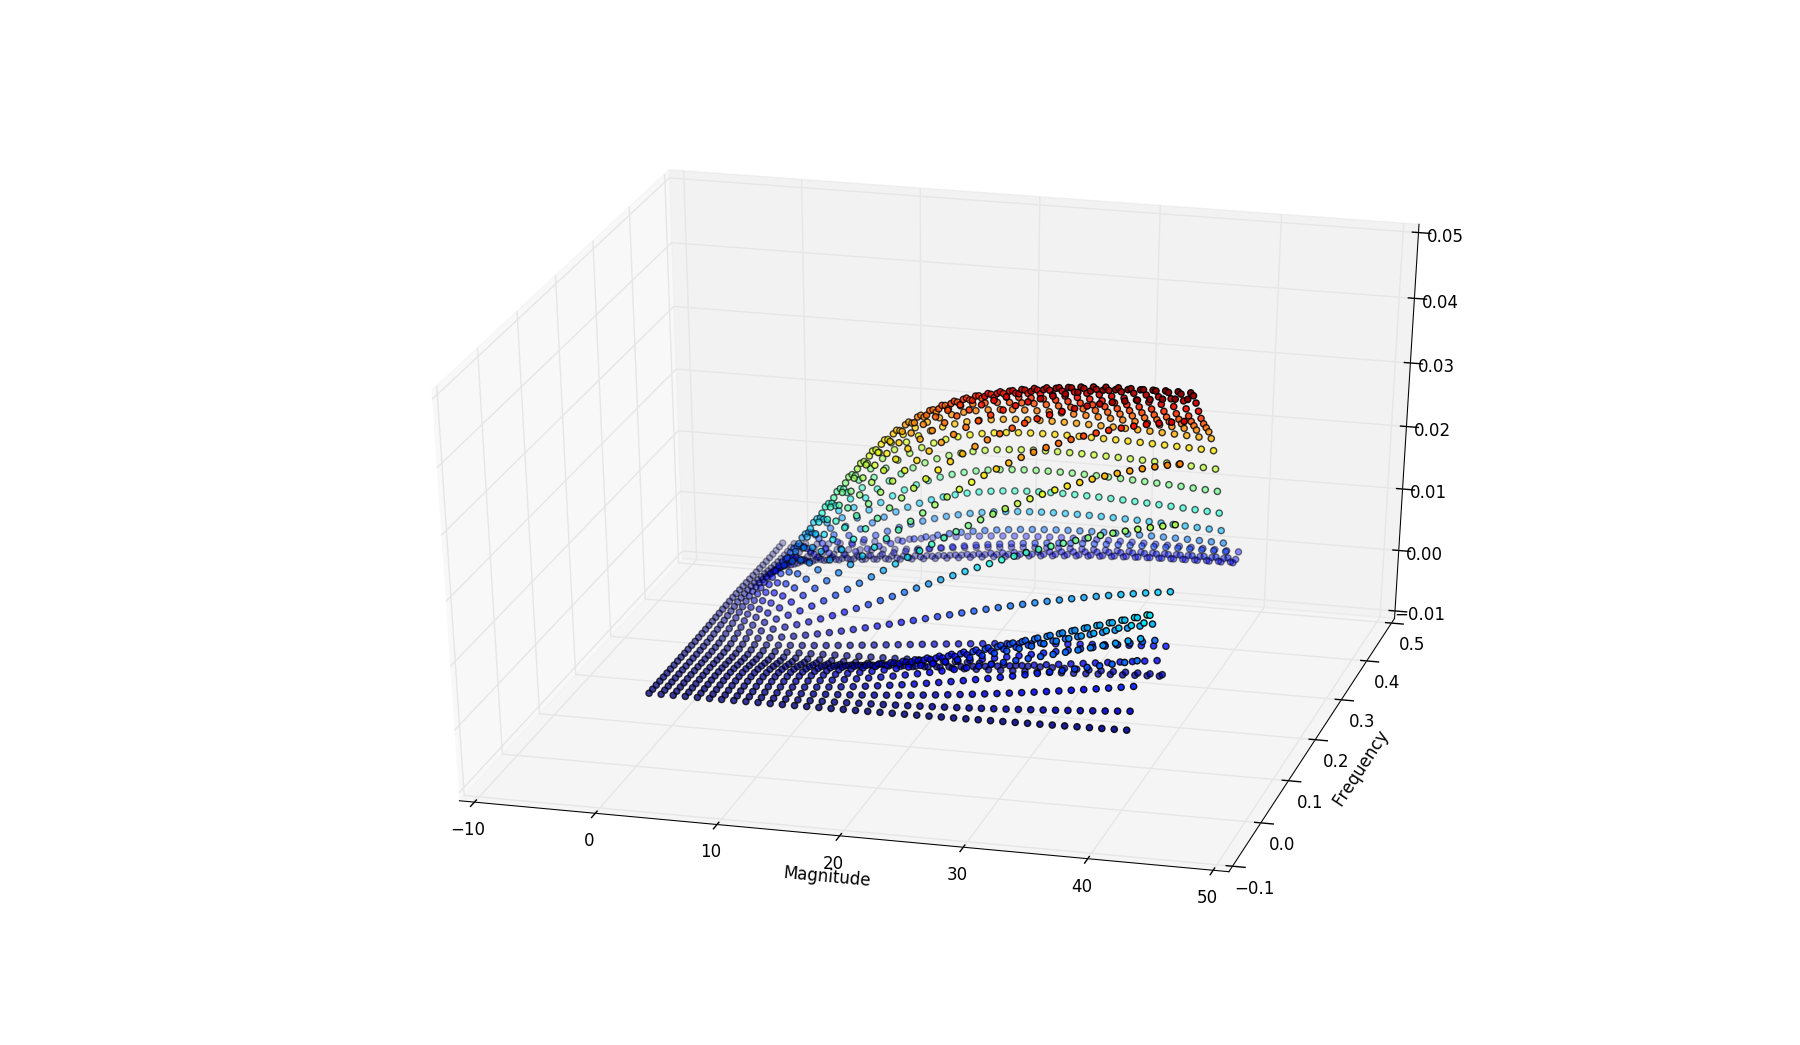
\includegraphics[width=\textwidth]{/home/cshome/j/jcampbell/Desktop/Thesis/Thesis/images/fixed_var_no_norm.png}
\caption{Variance computed from all possible examples, with no normalisation of the HSIC. Note that the peak is pronounced, however it incorrectly identifies the magnitude. \label{fixed_var_no_norm}}
\end{figure}

\begin{figure}[h]
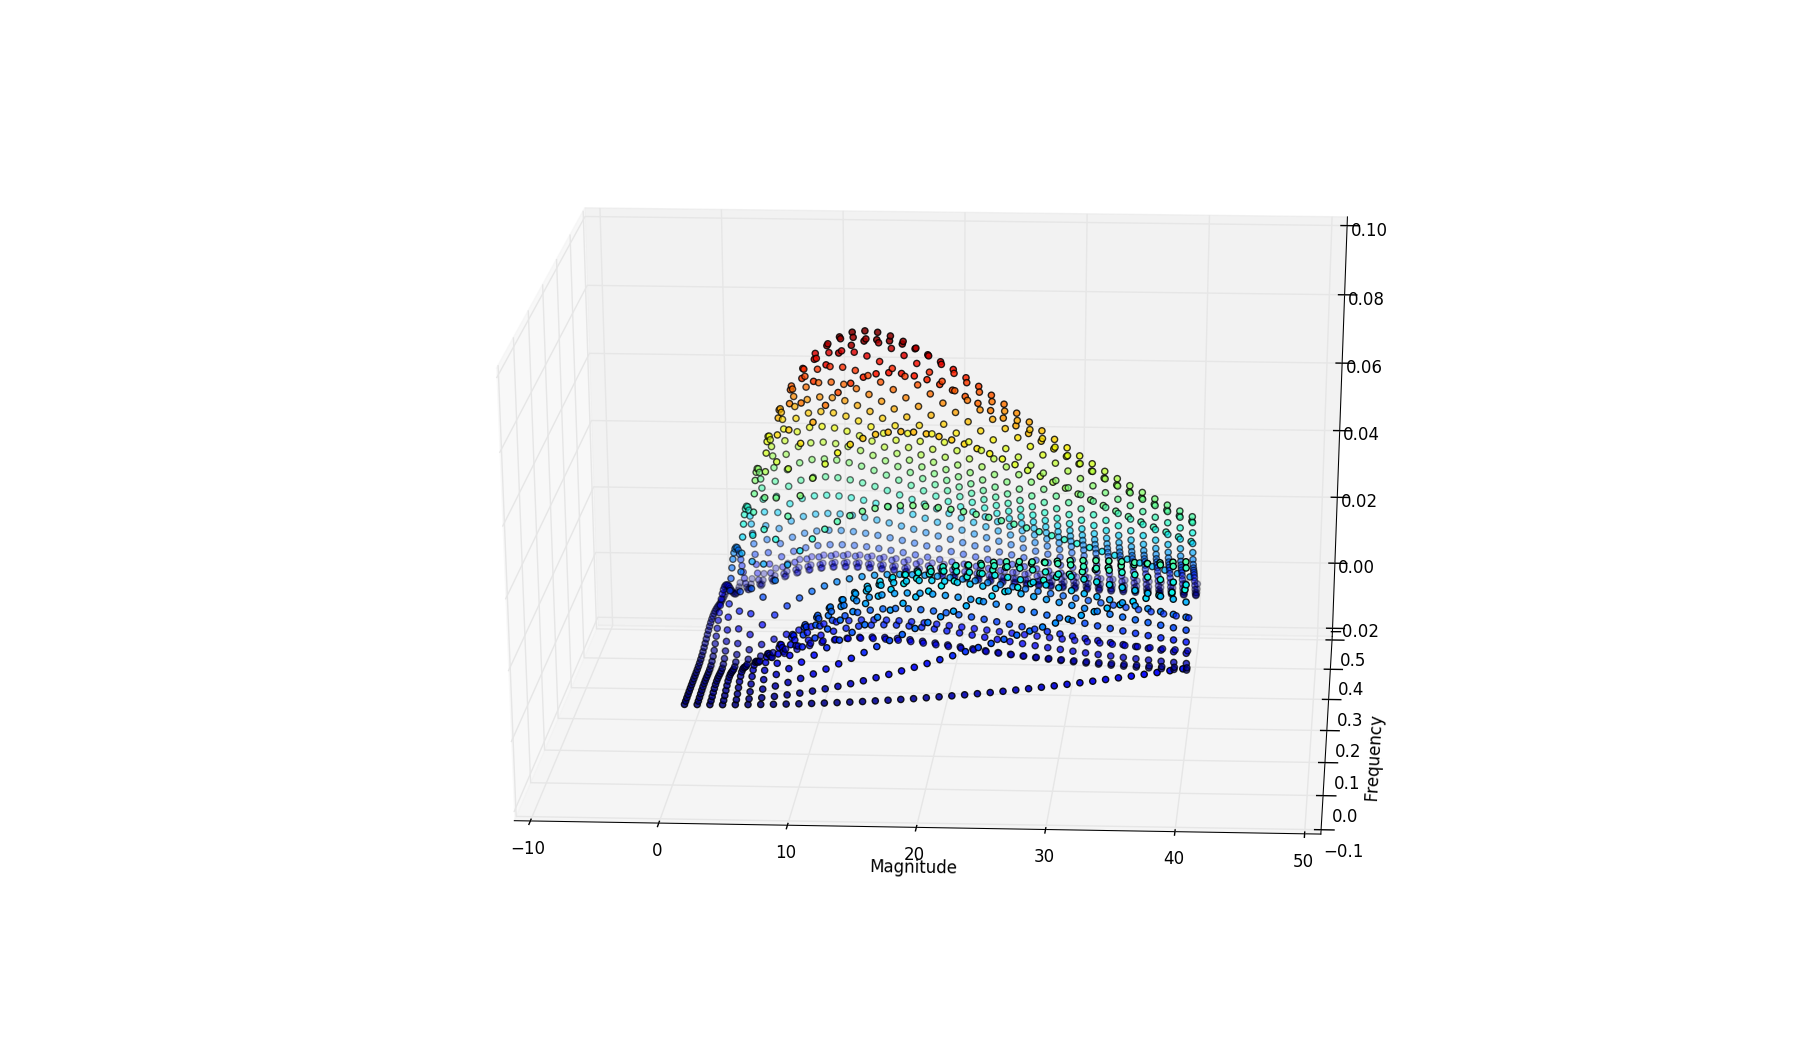
\includegraphics[width=\textwidth]{/home/cshome/j/jcampbell/Desktop/Thesis/Thesis/images/floating_var_no_norm.png}
\caption{Variance computed independently for every test example, with no normalisation of the HSIC. The peak is\label{floating_var_no_norm}}
\end{figure}

\begin{figure}[h]
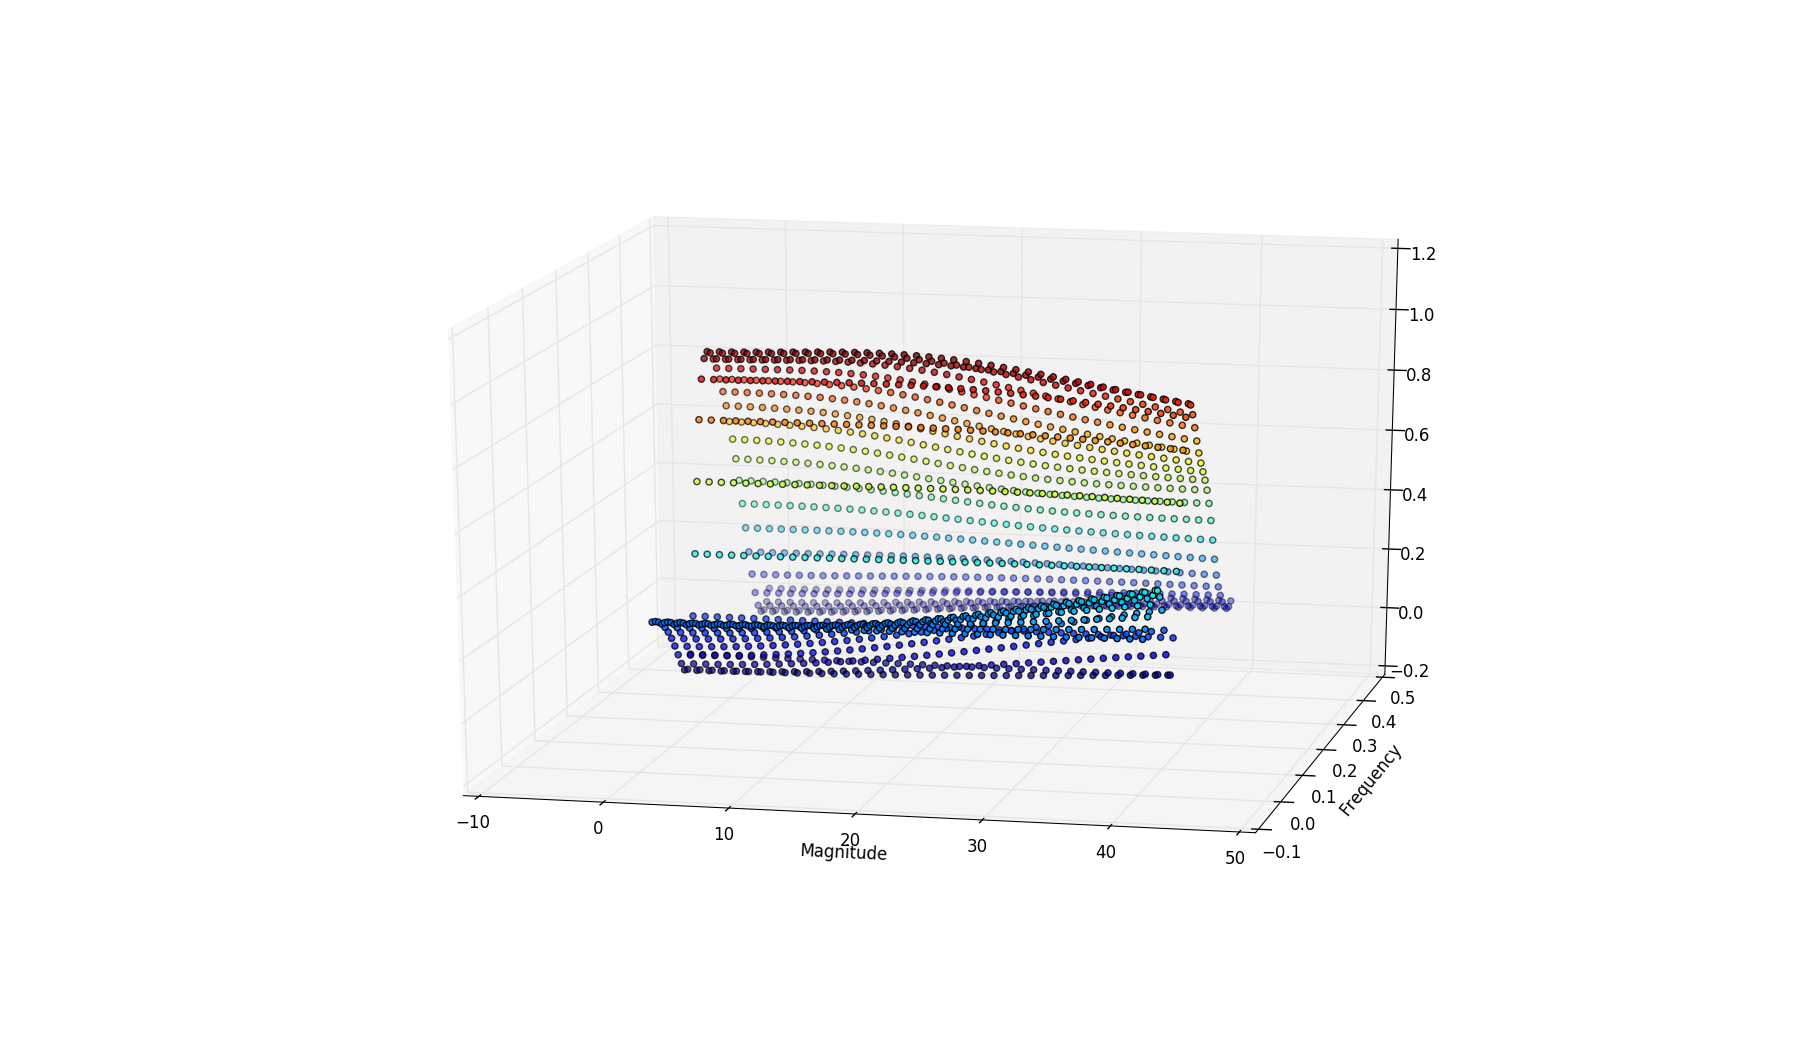
\includegraphics[width=\textwidth]{/home/cshome/j/jcampbell/Desktop/Thesis/Thesis/images/fixed_var_normalisation.png}
\caption{Variance computed from all possible examples, with normalisation of the HSIC.\label{fixed_var_normalisation}}
\end{figure}

\begin{figure}[h]
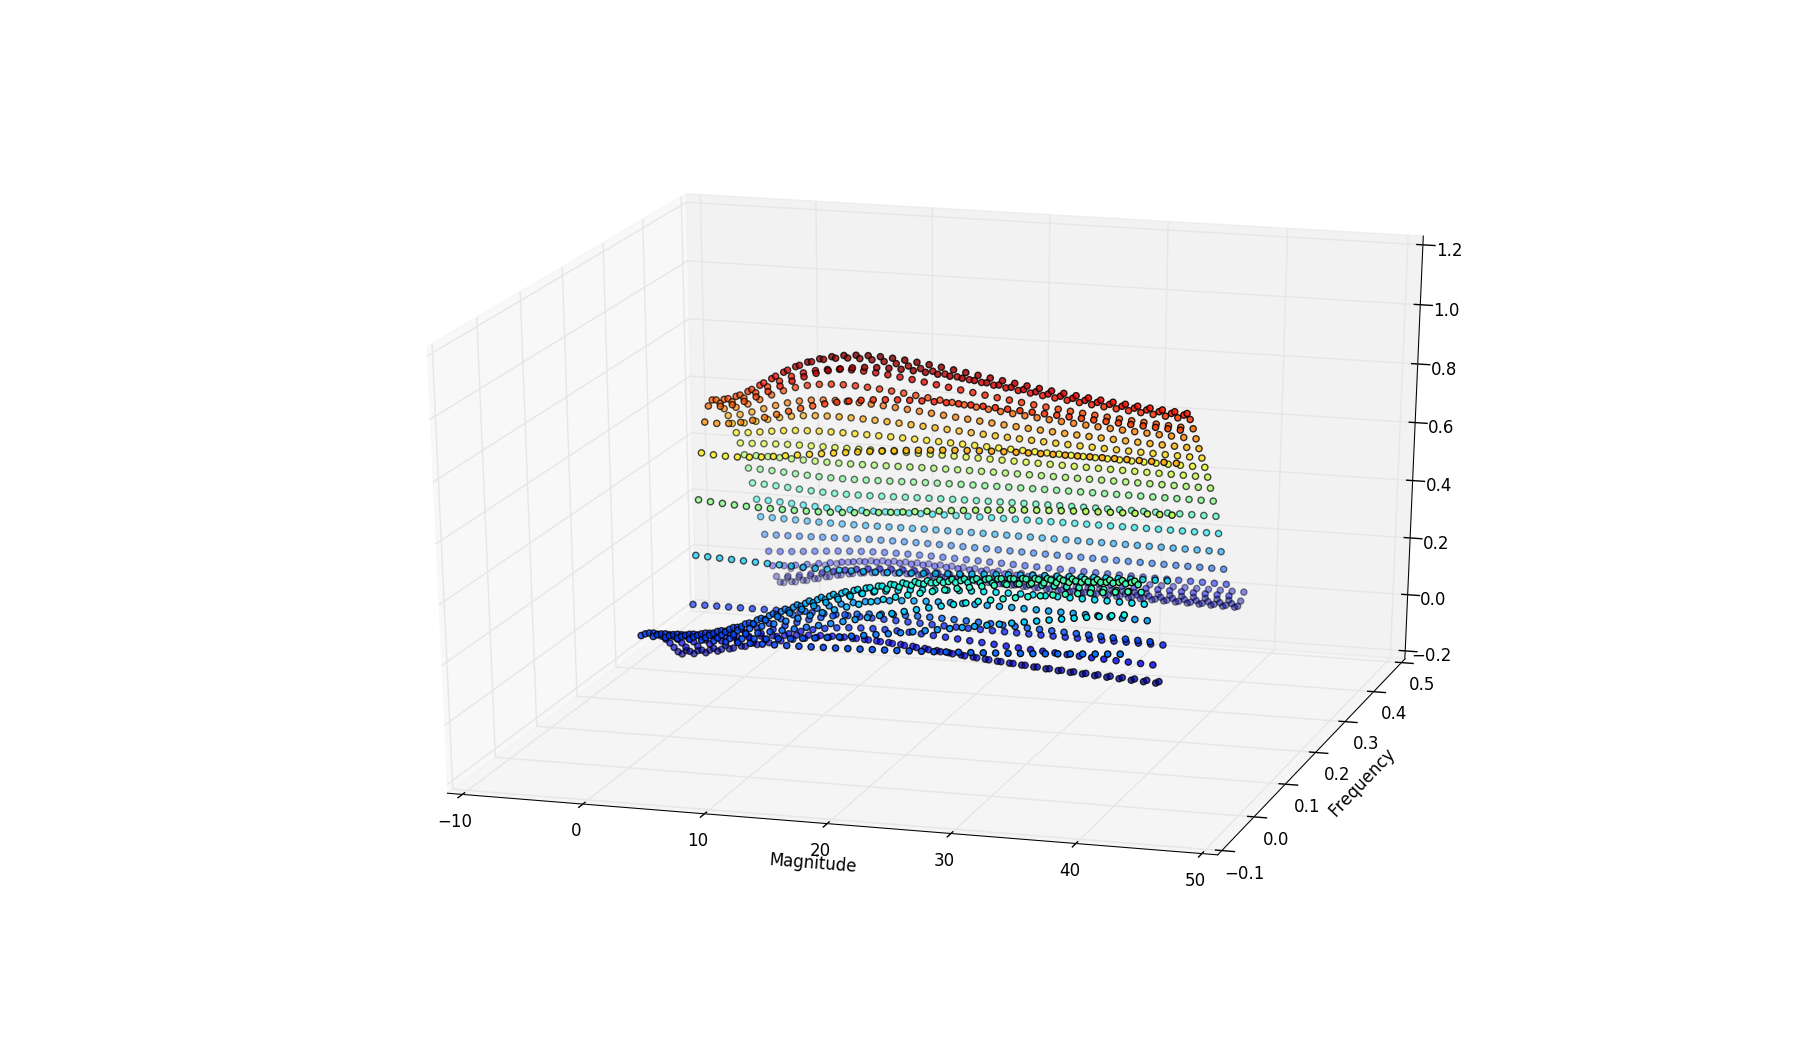
\includegraphics[width=\textwidth]{/home/cshome/j/jcampbell/Desktop/Thesis/Thesis/images/floating_var_normalisation.png}
\caption{\label{floating_var_normalisation}}
\end{figure}

\begin{figure}[h]
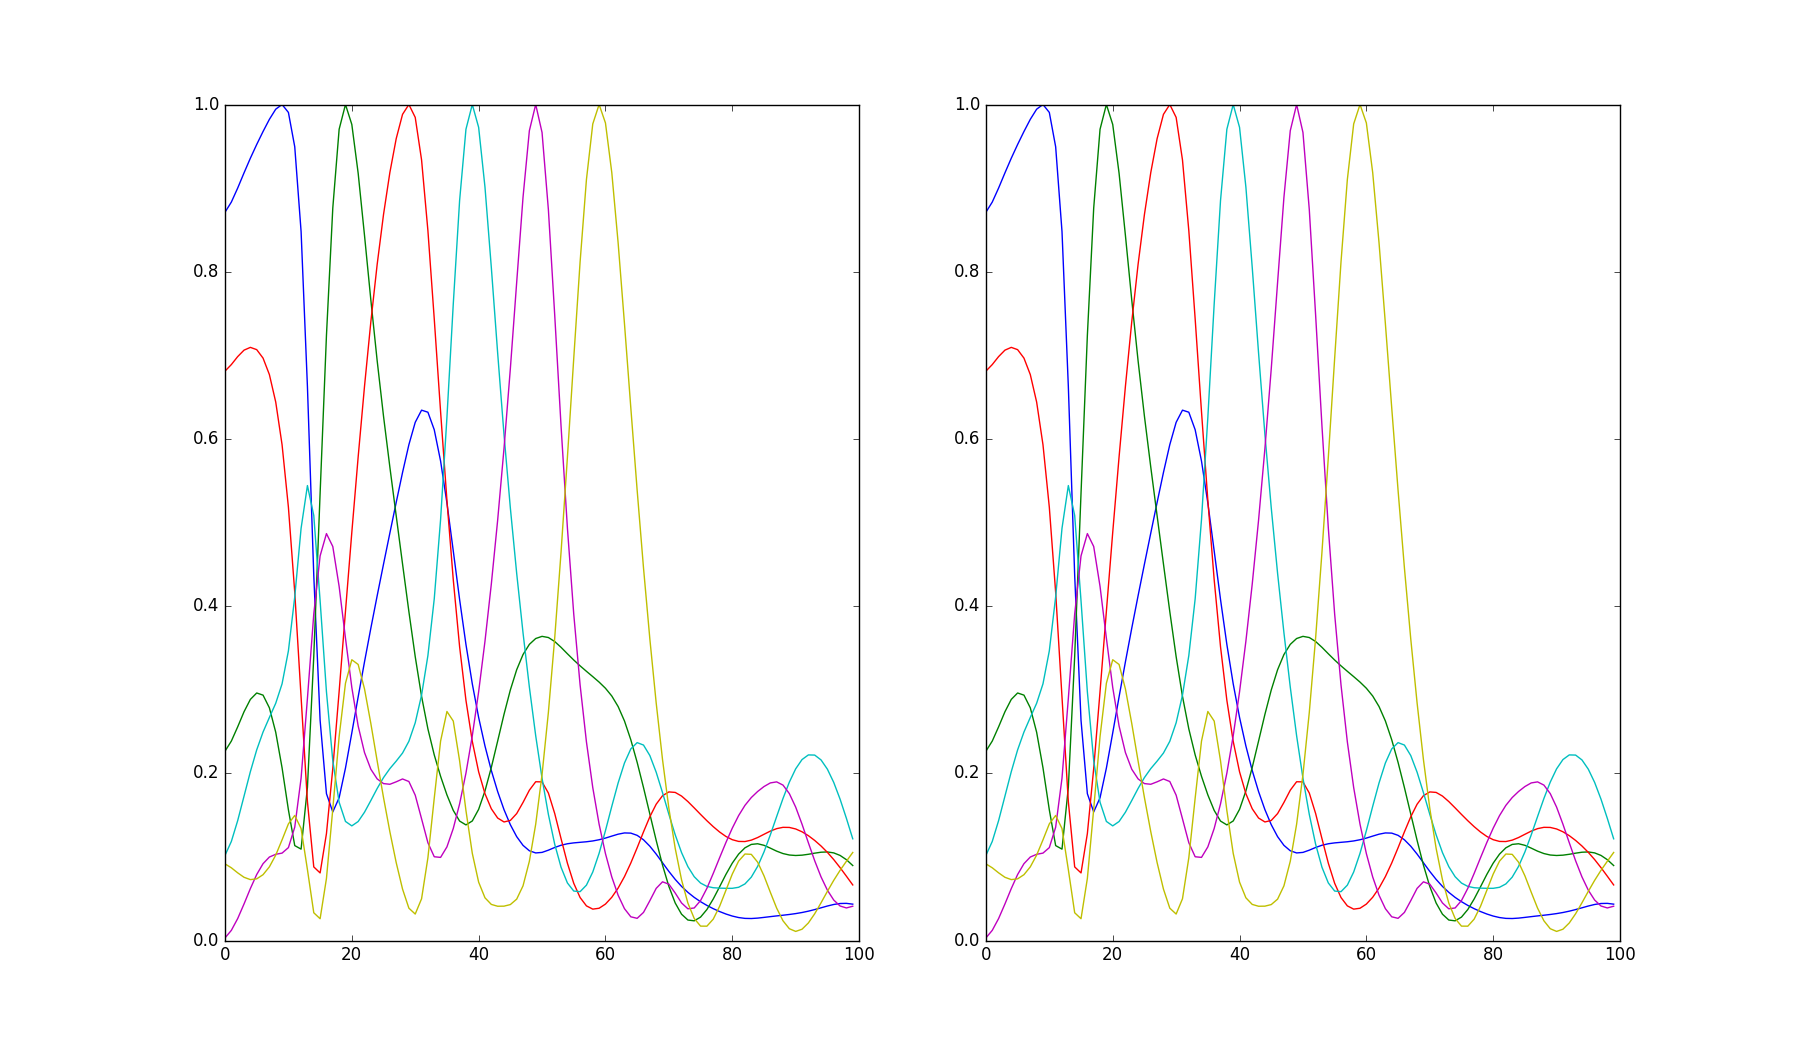
\includegraphics[width=\textwidth]{/home/cshome/j/jcampbell/Desktop/Thesis/Thesis/images/freq.png}
\caption{\label{freq}}
\end{figure}

\begin{figure}[h]
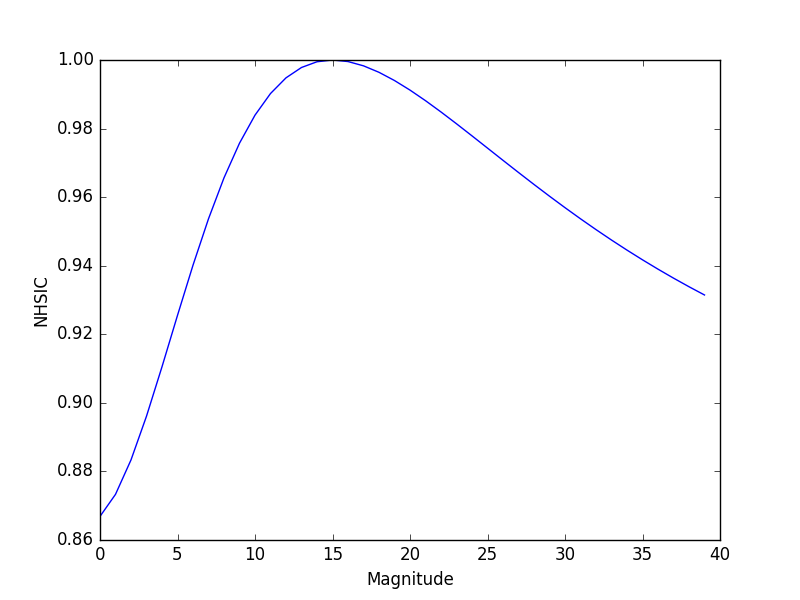
\includegraphics[width=\textwidth]{/home/cshome/j/jcampbell/Desktop/Thesis/Thesis/images/magnitude.png}
\caption{\label{magnitude}}
\end{figure}































\section{Action Recognition}

We turn now to the principle contribution of this chapter: to demonstrate that the Hilbert-Schmidt independence criterion can be used to match sequences of activities from motion capture data. As before we use the normalised HSIC, and estimate the covariance of the data for every pair of activities we wish to match. \\%One of the limitations of our method is that for any two action sequences we compare, we require that they are of equal length. We cannot match, for instance, a four second video of a person walking with an eight second video of a person walking.  This is less of a problem in cases where we are searching for instances of a reference action in a longer sequence, however we must account for the length of the input when matching two sequences in their entirety. This will be further discussed in section something.\\

In our first experiments we are given a short reference sequence of a walking motion, along with a longer video that contains various examples of both walking and climbing behaviour. The PCA transformed reference input is $X = \{x_0, x_1, ..., x_N\}$ where each $x_i$ is a $Q$ dimensional vector containing the $Q$ most significant components. We choose the number of PCA components, $Q$, for each experiment according to 

\begin{equation}
z = \frac{\sum_k^Q{\sqrt{e_k}}}{\sum_i^N{\sqrt{e_i}}} > 0.95
\end{equation}

\noindent where $e_i$ is the i\textit{th} eigenvalue of the principle components and $N$ is the number of samples. This allows us to choose the smallest number of principle components that explain more than $95\%$ of the variance of the data.\\

\begin{figure}[h]
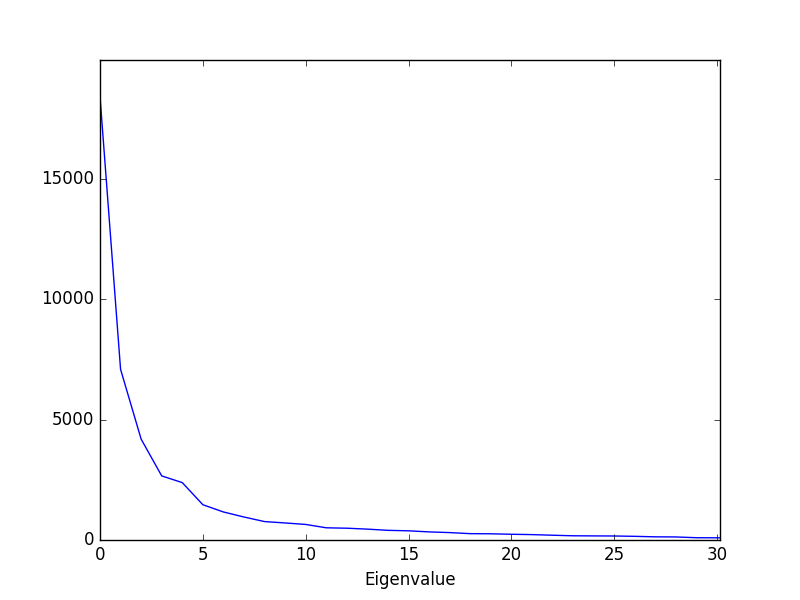
\includegraphics[width=\textwidth]{/home/cshome/j/jcampbell/Desktop/Thesis/Thesis/images/eigenvalues.png}
\caption{Plot of the square root of the eigenvalues of the data covariance matrix, in decreasing order. Only the first 30 values are shown for display purposes. \label{eigenvalues}}
\end{figure}

Our initial reference video is number 34 from subject 105 (herein referred to as 105/34) of the CMU Mocap database. Our test video is number two from subject one (herein referred to as 01/02) of the same database. In this experiment $Q$ is set to 29, as this is the larger of the $Q$ values for the two sequences. From 105/34 we selected a six second walking sequence as the reference motion, which corresponds to 720 mocap data samples. We use a number of reference sequences offset slightly from the starting point to reduce the sensitivity of our algorithm to changes in phase. Selected frames from the animated reference and test sequences are shown in Figs. \ref{105_34} and \ref{01_02} respectively. The frames in Fig. \ref{105_34} are indicative of all the subsequences used. The frames in Fig \ref{01_02} are from the closest matching subsequence from 01/02, i.e the subsequence that most resembles walking motion, according to our algorithm. Fig. \ref{ts_05} shows the results of running the NHSIC algorithm for a variety of offsets of the test sequence. Each sequence contains $M = 720$ data samples, however this is downsampled to $N = 200$ samples as the time complexity of the NHSIC algorithm has time complexity $O(N^2)$. There are two peaks in the results in Fig. \ref{ts_05}: at frame 45 and frame 104. The first peak correctly indicates the point in the sequence when the subject is walking, while the second peak refers to a subsequence for which the subject is climbing a set of stairs. These results are interesting as one would not typically not label a stair climbing sequence as walking, which raises an interesting problem with our algorithm: we currently have neither an objective measure of success, nor do we have any means of selecting against negative examples. These two problems are discussed after the presentation of the results. These results do, however, clearly demonstrates the strength of the Hilbert-Schmidt independence criterion to match sequences which share common underlying characteristics.% To further demonstrate the strength of the NHSIC, Fig. \ref{ts_09_expanded} shows an expanded section of results from Fig. \ref{ts_09}, which highlights the twin peaks at frames 105 and 108, with a much lower result at frame 107, between them. This drop corresponds to a subsequence where the subject climbs the stairs, waits, and then climbs back down. The peaks on either side of this drop refer to subsequences where the subject is predominantly climbing either up or down the stairs. \\

We further tested our algorithm with the same reference sequence (105/34) but with a different test sequence: video 15 from subject 86 (86/15) of the CMU mocap database. In this video the subject walks in a small circle for a short period of time, sits down, waves their arms, makes a number of miscellaneous actions, then stands and walks in a small circle again. The results of running our algorithm under the same conditions as the previous experiment are shown in Fig. \ref{ts_08}, where we can clearly see the strong match at the start of the sequence (frames 0 - 22), and at the end of the sequence (frame 210). These results also show a weaker match at frames 93 - 103. This weaker match occurs when the subject is sitting and makes a brushing motion with their arm. Since this motion is isolated (does not appear in conjunction with other motions) it is being labelled as similar to the reference walking motion. This highlights the issue with the NHSIC for identifying false positives and is discussed further in the future work section. \\

Our final experiment of this section was on sequence eight from subject 86 (86/08) of the CMU mocap database. This subject initially walks, then performs a series of squats, twists, cyclical arm motions, and kicks. The subject then runs for a short period of time before performing punching actions and then walking again. Our algorithm identified approximately four motions that closely resembled walking. Two of these are indeed walking motions, however it also identifies the running period and kicking period as walking. The walking periods were the two closest matches, followed by the running period and then the kicking action. 

\begin{figure}
\centering
\begin{subfigure}{0.24\textwidth}
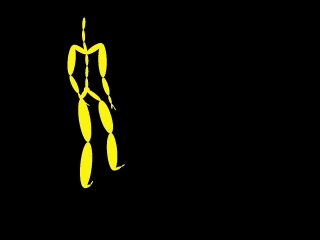
\includegraphics[width=\textwidth]{/home/cshome/j/jcampbell/Desktop/Thesis/Thesis/images/105_34/105.png}
\end{subfigure}
\begin{subfigure}{0.24\textwidth}
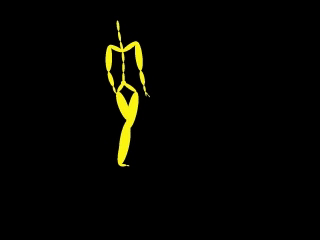
\includegraphics[width=\textwidth]{/home/cshome/j/jcampbell/Desktop/Thesis/Thesis/images/105_34/130.png}
\end{subfigure}
\begin{subfigure}{0.24\textwidth}
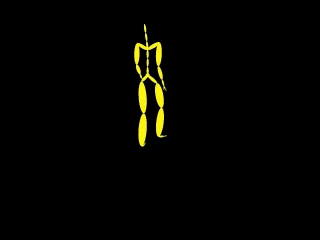
\includegraphics[width=\textwidth]{/home/cshome/j/jcampbell/Desktop/Thesis/Thesis/images/105_34/155.png}
\end{subfigure}
\begin{subfigure}{0.24\textwidth}
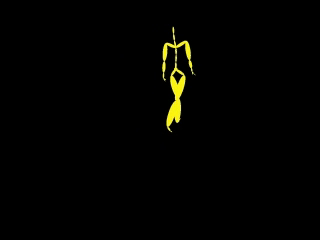
\includegraphics[width=\textwidth]{/home/cshome/j/jcampbell/Desktop/Thesis/Thesis/images/105_34/180.png}
\end{subfigure}

\begin{subfigure}{0.24\textwidth}
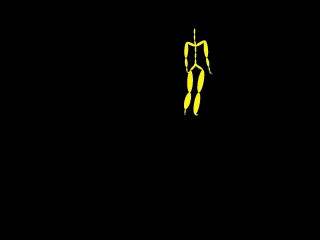
\includegraphics[width=\textwidth]{/home/cshome/j/jcampbell/Desktop/Thesis/Thesis/images/105_34/205.png}
\end{subfigure}
\begin{subfigure}{0.24\textwidth}
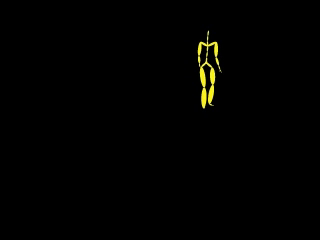
\includegraphics[width=\textwidth]{/home/cshome/j/jcampbell/Desktop/Thesis/Thesis/images/105_34/230.png}
\end{subfigure}
\begin{subfigure}{0.24\textwidth}
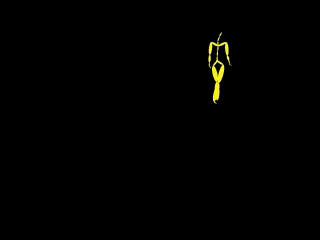
\includegraphics[width=\textwidth]{/home/cshome/j/jcampbell/Desktop/Thesis/Thesis/images/105_34/255.png}
\end{subfigure}
\begin{subfigure}{0.24\textwidth}
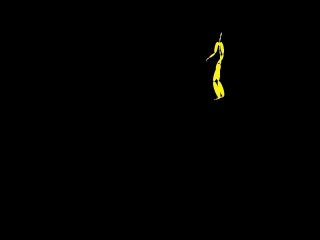
\includegraphics[width=\textwidth]{/home/cshome/j/jcampbell/Desktop/Thesis/Thesis/images/105_34/285.png}
\end{subfigure}
\caption{ Selected frames from the reference sequence of 105/34.   \label{105_34}}
\end{figure}

\begin{figure}
\centering
\begin{subfigure}{0.24\textwidth}
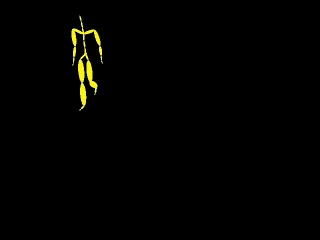
\includegraphics[width=\textwidth]{/home/cshome/j/jcampbell/Desktop/Thesis/Thesis/images/01_02/335.png}
\end{subfigure}
\begin{subfigure}{0.24\textwidth}
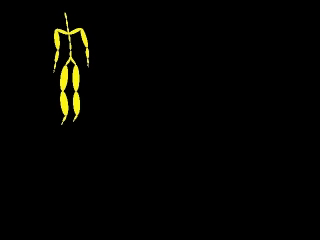
\includegraphics[width=\textwidth]{/home/cshome/j/jcampbell/Desktop/Thesis/Thesis/images/01_02/360.png}
\end{subfigure}
\begin{subfigure}{0.24\textwidth}
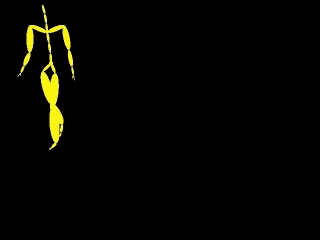
\includegraphics[width=\textwidth]{/home/cshome/j/jcampbell/Desktop/Thesis/Thesis/images/01_02/385.png}
\end{subfigure}
\begin{subfigure}{0.24\textwidth}
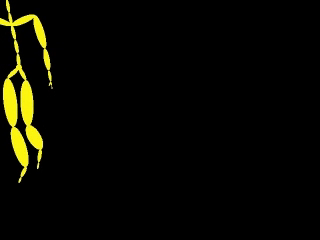
\includegraphics[width=\textwidth]{/home/cshome/j/jcampbell/Desktop/Thesis/Thesis/images/01_02/410.png}
\end{subfigure}

\begin{subfigure}{0.24\textwidth}
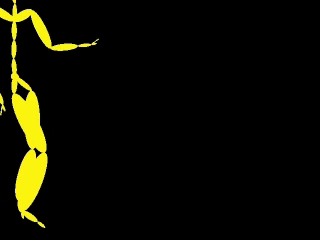
\includegraphics[width=\textwidth]{/home/cshome/j/jcampbell/Desktop/Thesis/Thesis/images/01_02/435.png}
\end{subfigure}
\begin{subfigure}{0.24\textwidth}
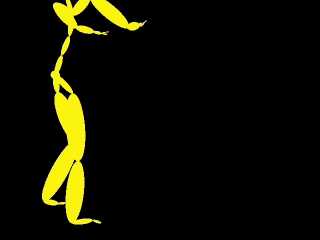
\includegraphics[width=\textwidth]{/home/cshome/j/jcampbell/Desktop/Thesis/Thesis/images/01_02/460.png}
\end{subfigure}
\begin{subfigure}{0.24\textwidth}
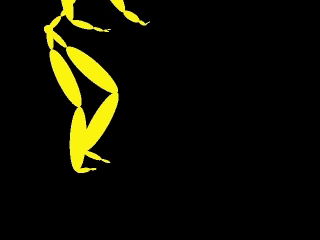
\includegraphics[width=\textwidth]{/home/cshome/j/jcampbell/Desktop/Thesis/Thesis/images/01_02/485.png}
\end{subfigure}
\begin{subfigure}{0.24\textwidth}
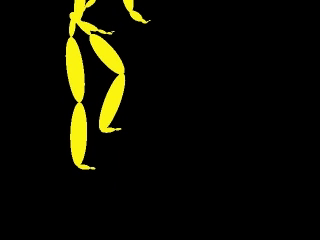
\includegraphics[width=\textwidth]{/home/cshome/j/jcampbell/Desktop/Thesis/Thesis/images/01_02/500.png}
\end{subfigure}
\caption{Selected frames from the subsequence of 01/02 that matches the reference sequence in 105/34.\label{01_02}}
\end{figure}

\begin{figure}[h]
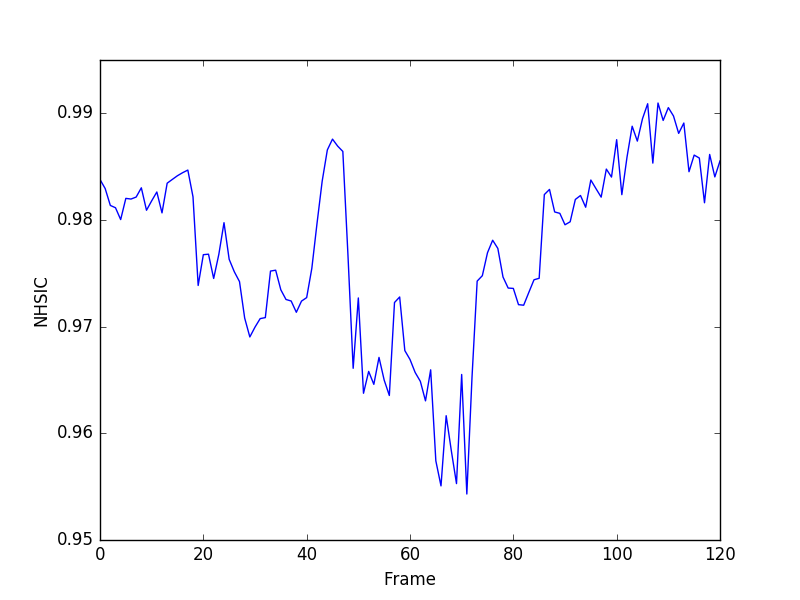
\includegraphics[width=\textwidth]{/home/cshome/j/jcampbell/Desktop/Thesis/Thesis/images/ts_09.png}
\caption{Activity recognition results for 01/02. Note the strong peak at frame 45 (walking) and the broader peak at frames 104 - 112 (climbing stairs).\label{ts_09}}
\end{figure}

%\begin{figure}[h]
%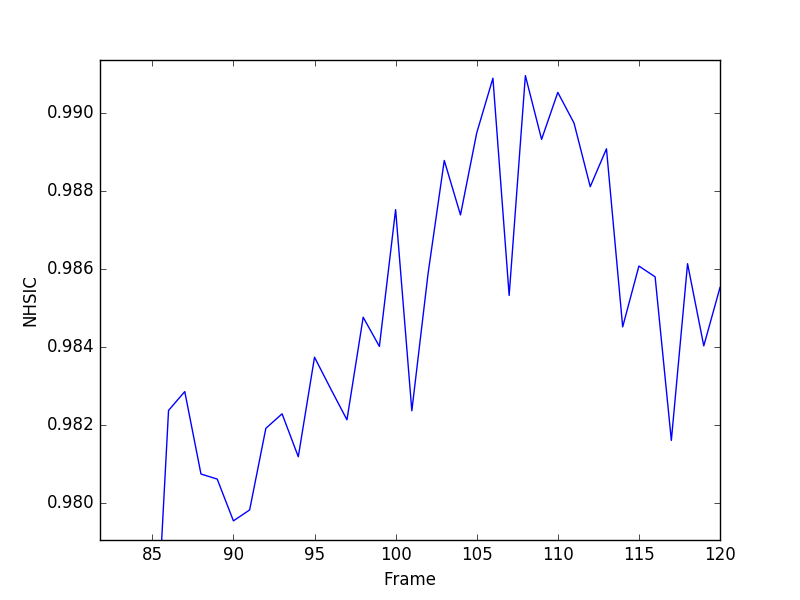
\includegraphics[width=\textwidth]{/home/cshome/j/jcampbell/Desktop/Thesis/Thesis/images/ts_09_expanded.png}
%\caption{Expanded results from Fig. \ref{ts_09} for frames 85 - 120. The subject begins climbing the stairs at frame 104, reaches the top at frame  \label{ts_09_expanded}}
%\end{figure}

\begin{figure}[h]
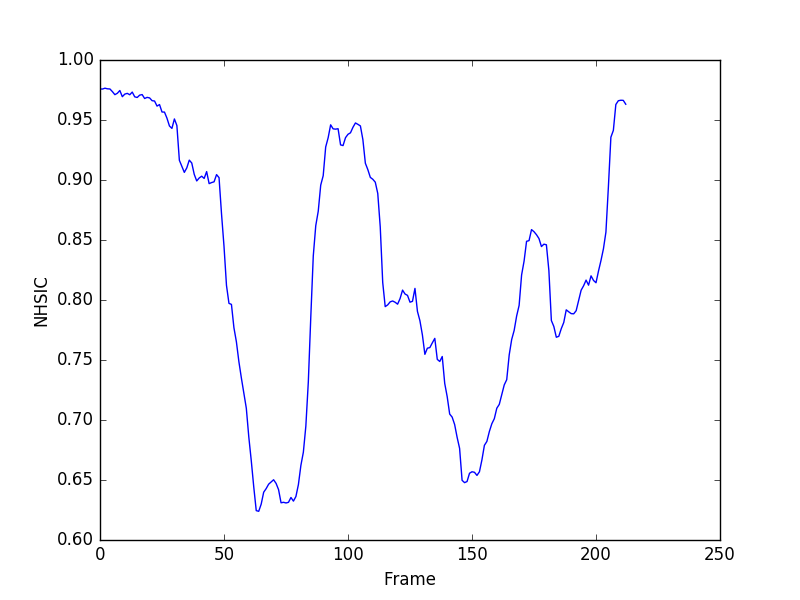
\includegraphics[width=\textwidth]{/home/cshome/j/jcampbell/Desktop/Thesis/Thesis/images/ts_08.png}
\caption{\label{ts_08}}
\end{figure}


\begin{figure}[h]
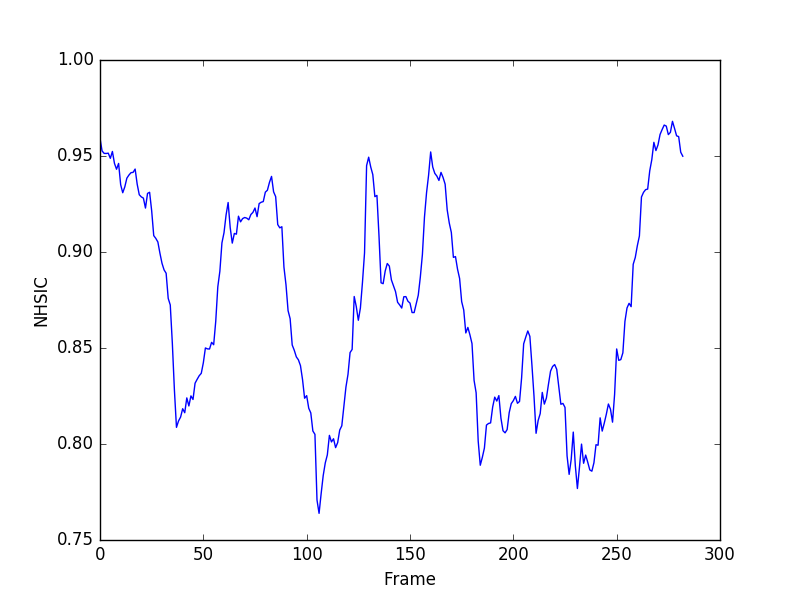
\includegraphics[width=\textwidth]{/home/cshome/j/jcampbell/Desktop/Thesis/Thesis/images/ts_10.png}
\caption{\label{ts_10}}
\end{figure}

\begin{figure}[h]
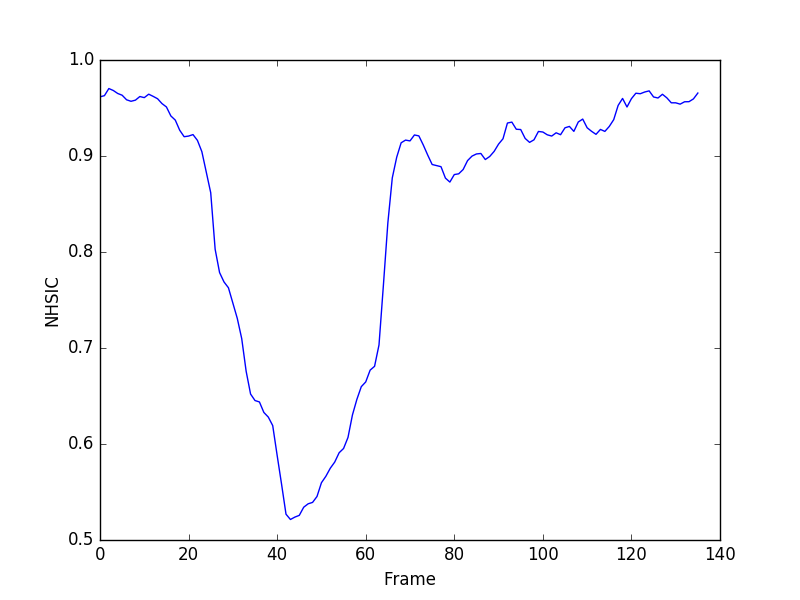
\includegraphics[width=\textwidth]{/home/cshome/j/jcampbell/Desktop/Thesis/Thesis/images/ts_11.png}
\caption{\label{ts_11}}
\end{figure}




























\section{Temporal Synchronisation}

There are often times when two vides of an activity will not be temporally aligned, for example in film making. In the film industry the term \textit{shot} is used to denote a short sequence of continuous activity which is not broken by a cut, typically on the order of 1000 frames. It is common for multiple cameras to record each shot, as well as infrared cameras if motion capture technology is being employed. Motion capture systems typically contain their own dedicated hardware temporal synchronisation frameworks, while an additional hardware synchronisation system is employed for the remaining cameras. Hardware synchronisation methods are occasionally used for filming outdoors, however they are often costly and require time to setup for each shoot. Hardware synchronisation methods are therefore inaccessible for amateur cinematographers, and for unplanned, ad hoc recording scenarios. In these situations it is therefore highly likely that the activity recorded from each camera will not be synchronised in time. Furthermore, even if hardware synchronisation has been used, once a shot has been captured it will often be sent to an editorial team, who may perform alterations to the shot which renders the timestamps incorrect. The original and the modified shots will therefore require manual synchronisation to align them again. Manual synchronisation is typically performed by searching for high frequency events such as footfalls, eyeblinks, or when any two items connect. This obviously introduces problems when there is very little scene activity, or when there are no high frequency components. This could occur in tracking shots that produce a sweeping motion, or for shots in which any activity is very smooth, for example a car driving along a street. \\

It is vitally important that multiple views of a shot are aligned in time. In live action films it is critical to know when to be able to switch between views, while in films that contain visual effects elements the multiple views are used as input to motion reconstruction pipelines, stereo reconstruction pipelines, and as raw input for artists manually creating creatures and scenes. \\

\subsection{Matching mocap with Iimage data}

One of the strengths of the HSIC is it can theoretically find all the functional dependencies between two random variables. Critically, this means that we can use the HSIC to match data from disparate sensing modalities, i.e. between mocap data and image data. In some film production settings it may be necessary to find the temporal offset between the motion capture data of a scene, and some video of that scene. We therefore tested our algorithm under these settings, and show that it is possible to synchronise 

\section{Activity Clustering}

\subsection{}
